\documentclass[10pt]{article}

%%% These are some packages that are useful
\usepackage{amsmath,amssymb, amscd,amsbsy, amsthm, enumerate}
\usepackage[export]{adjustbox}
\usepackage{lastpage}
\usepackage[top=1in, bottom=1in, left=1in, right=1in]{geometry}
\usepackage[unicode]{hyperref}
\usepackage{tikz, pgfplots, xcolor, fancyhdr}
\usepackage{multicol,caption}
\usepackage{lipsum}
\usepackage[version=4]{mhchem}
\usepackage{float}

%%% Page formatting
%\setlength{\headsep}{30pt}
\setlength{\textheight}{9in}
\newcommand{\tab}{\hspace{1cm}}
%\setlength{\parindent}{25pt}

\title{Fountains Of The Deep}
\author{Antonius Torode}

%%% Header and Footer Info
\pagestyle{fancy}
\fancyhead[L]{{\large Template - \textbf{Change 03}}}
\fancyhead[C]{\today}
\fancyhead[R]{Name: Antonius Torode}


\fancyhf{} % sets both header and footer to nothing
\renewcommand{\headrulewidth}{0pt}
% your new footer definitions here

\fancyfoot[L]{}
\fancyfoot[C]{}
\fancyfoot[R]{\thepage\ of \pageref{LastPage}}

% Used to define spacing and format of References
\let\OLDthebibliography\thebibliography
\renewcommand\thebibliography[1]{
	\OLDthebibliography{#1}
	\setlength{\parskip}{0pt}
	\setlength{\itemsep}{0pt plus 0.3ex}
}

\newenvironment{Figure}
  {\par\medskip\noindent\minipage{\linewidth}}
  {\endminipage\par\medskip}


%%% Document Starts now
\begin{document}

\maketitle
\thispagestyle{fancy}


\begin{abstract}
This paper examines the feasibility of the biblical great flood by estimating the volume of water required to cover all land, including mountain peaks. A simple spherical volume calculation indicates that flooding the Earth to the height of Mount Everest would require and overestimate of approximately \textit{three} times the volume of Earth’s oceans. While conventional scientific understanding asserts that Earth’s surface water is nearly limited to the oceans, recent geological research reveals substantial water reservoirs deep within the Earth’s mantle, supporting scriptural references to “the fountains of the deep.” By combining quantitative analysis, scripture, and contemporary science, this study presents a coherent perspective that reconciles the flood narrative with current geological knowledge.
\end{abstract}

\begin{multicols}{2}

While reading through the story of Noah and the great flood, an important question arises. Does the Earth have enough water to allow for the great flood? Is there enough water on Earth to cover all the land and all the mountain tops? A brief search online shows numerous articles, lengthy forum discussions, and entire sites asserting that this is just not possible. Most of these say same compelling thing - there's just not enough water on the Earth. Naturally, as a skeptic, I put it to the test.

How much water would be required to flood the Earth? Estimating this requires a relatively simple calculation. This estimate requires two assumptions. The first is that Earth is spherical - which is a reasonable approximation, especially on this scale. The second assumption is that there are about as many hills and mountains as there are valleys and ravines (assuming terrain averages out to sea level). We can ignore existing bodies of water below sea level, as they are already filled; we only need to account for the volume required to raise water from sea level to the highest elevations. This is actually an over-estimation (of how much water would be needed), as there is far more land above sea level than there is below - which is good because it provides more of a steel man case to test against\footnote{A mathematical tip when performing rough estimates like this is to always overestimate in a way that works against your expected result. That ensures that you can be more confident (than otherwise) of your final results if they support your hypothesis.}. In reality, much of the space above sea level is already occupied by land, so it would \textit{not} require water to fill that space in.

\begin{Figure}
	\centering
	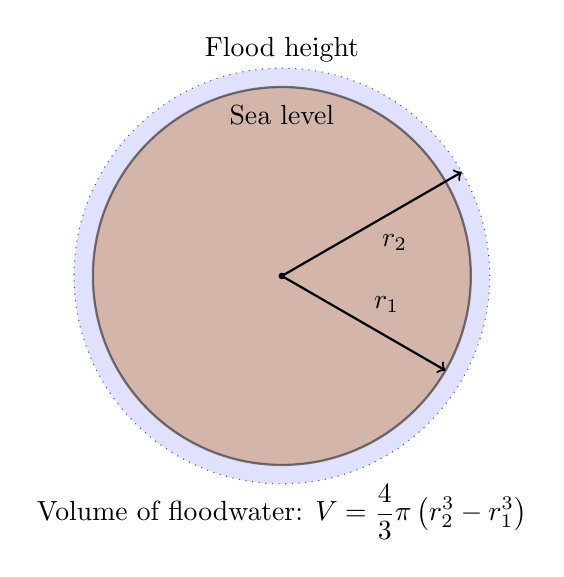
\begin{tikzpicture}[scale=1.2]
	  % Radii
	  \def\Rcore{2}      % Inner radius (Sea Level)
	  \def\Rsurface{2.2} % Outer radius (Mount Everest or animal elevation)
	
	  % Draw outer shell (Flood height)
	  \draw[dotted, fill=blue!20, opacity=0.6] (0,0) circle (\Rsurface);
	  
	    % Draw inner Earth circle (Sea Level)
	    \draw[thick, fill=brown!90, opacity=0.5] (0,0) circle (\Rcore);
	
	  % Center point
	  \fill (0,0) circle (1pt) node[below left] {};
	
	  % Inner radius label at -30 degrees
	  \draw[->, thick] (0,0) -- ({\Rcore*cos(-30)}, {\Rcore*sin(-30)})
	    node[midway, above right] {$r_1$};
	
	  % Outer radius label at +30 degrees
	  \draw[->, thick] (0,0) -- ({\Rsurface*cos(30)}, {\Rsurface*sin(30)})
	    node[midway, below right] {$r_2$};
	
	  % Arc labels
	  \node at (0,1.7) {Sea level};
	  \node at (0,2.4) {Flood height};
	
	  % Volume label
	  \node at (0,-2.5) {
	    Volume of floodwater: 
	    $\displaystyle V = \frac{4}{3}\pi \left(r_2^3 - r_1^3\right)$
	  };
	\end{tikzpicture}
	
	{\footnotesize Figure 1. Simplified 2D diagram illustrating the volume calculation for floodwater between sea level ($r_1$) and flood height ($r_2$).}
\end{Figure}

The total volume of water needed for the flood can then be calculated by using the formula for spherical volume, and taking the difference of the volume from the top of the tallest mountain\footnote{Genesis 7:20 states ``The waters prevailed fifteen cubits upward, and the mountains were covered.'' This suggests this value should be slightly \textit{higher} than the tallest mountain (by a few meters), but this distance is negligible on these scales alongside the other approximations.} and at sea level (see figure 1). The radius of Earth is about 6378.0 km. The height of mount Everest is about 8.8 km above sea level, which puts its peak at a distance of 6386.8 km from the center of the earth. Using these values, we can calculate the amount of water needed to flood the earth (covering all the mountaintops) as ``$\approx 3 \times $ volume of Earth's oceans $(1.332 \times 10^9)$ km$^3$'' according to the Wolfram Alpha computational engine (see figure 2).

\begin{Figure}
	\centering
		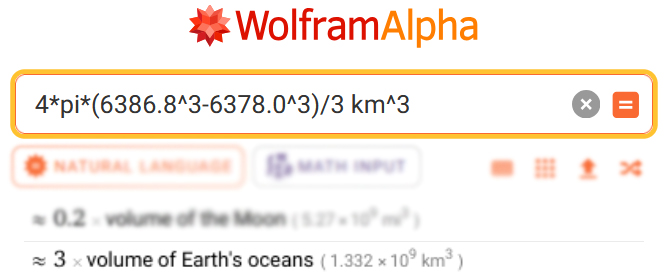
\includegraphics[width=\textwidth]{wolfram_edited.jpg}
	{\footnotesize Figure 2. The calculation of total floodwater on earth using the approximations outlined throughout this paper. This image shows the actual output of the calculation as displayed by Wolfram Alpha \cite{WolframAlpha}, edited only to remove other (irrelevant) conversions and comparisons (for sake of figure space).}
\end{Figure}

Thus, it would take approximately \textit{three} times the volume of Earth's oceans as extra water to flood the Earth. So, how much water is on Earth? In 2019, the United States Geological Survey (USGS) published an article titled ``How Much Water is There on Earth?'' They discuss the spread of water on Earth and state,
\begin{quotation}
\noindent``the oceans hold about 96.5 percent of all Earth's water \cite{ocean water}.'' 
\end{quotation}
In other words, almost all of the Earth' water is in the oceans. This presents a significant problem. Does that mean the flood described in the Bible could not have happened? The key to understanding how this is possible is given to us within the scriptures themselves. First, when the flood is occurring:
\begin{quotation}
\noindent``In the six hundredth year of Noah’s life, in the second month, the seventeenth day of the month, on that day all the \textit{fountains of the great deep} were broken up, and the windows of heaven were opened.'' - Genesis 7:11
\end{quotation}
Later, when the flood was over:
\begin{quotation}
\noindent``\textit{The fountains of the deep} and the windows of heaven were also stopped, and the rain from heaven was restrained.'' - Genesis 8:2
\end{quotation}
The key phrase here is \textit{the fountains of the deep}. This implies that the water came from deep within the Earth.

There's an obvious problem with the previous article that was mentioned. Fortunately, they list all of the sources they use, which includes a table from 1993, observatory information (visible water only), and data they already had from 1984. This article was published in 2019, but it fails to use scientific discoveries from \textit{five years} prior.

In 2014, an article was published in \textit{Science} (an academic journal) which talked about the Earth's mantle transition zone (410 to 660 km below the surface) acting as a huge reservoir of water \cite{mantle water}. The Smithsonian Science Education Center even said in an article that the oceans themselves may have simple seeped out of the core of Earth \cite{ocean below feet}. The Brookhaven National Laboratory discusses this discovery in detail. They say this is a long speculated result where the water in Earth's core is actually trapped in the crystalline mineral structures - neither as liquid, ice, or vapor \cite{deep earth water}. It's not known the exact amount of water stored in Earth's core, but they state one quote which I found right after my little calculation above.

\begin{quotation}
\noindent``If just one percent of the weight of mantle rock located in the transition zone is \ce{H2O}, that would be equivalent to nearly \textit{three} times the amount of water in our oceans, the researchers said \cite{deep earth water}.''
\end{quotation}

Despite there being countless sources suggesting that the great flood could not be possible, it's clear to see that this is simply yet another case of science not quite catching up to the Bible. A simple calculation shows it would take \textit{three} times the water in all of Earth's oceans to cause the great flood. Even though some scientists say the oceans make up almost all our water, the scriptures tell us to look deeper. Recent discoveries show us that \textit{the fountains of the deep} aren't just words on a page - but reality. When we study these things ourselves, we see repeatedly that the Bible holds mysteries science is still catching up to.




\begin{thebibliography}{9}
	{\footnotesize
		
	\bibitem{WolframAlpha} WolframAlpha. Computational Knowledge Engine: \url{https://www.wolframalpha.com}
	
	\bibitem{ocean water} United States Geological Survey (USGS), Water Science School, ``How Much Water is There on Earth?'' November 13, 2019  \url{https://www.usgs.gov/special-topics/water-science-school/science/how-much-water-there-earth}
		
	\bibitem{mantle water} Brandon Schmandt et al.,``Dehydration melting at the top of the lower mantle.'' Science344, 1265-1268(2014). \url{https://www.science.org/doi/10.1126/science.1253358}
		
	\bibitem{ocean below feet} Julia Rothchild, ``Is there An Ocean Below Your Feet?'' \url{https://ssec.si.edu/stemvisions-blog/there-ocean-below-your-feet}
		
	\bibitem{deep earth water} Karen McNulty Walsh, ``New Evidence for Oceans of Water Deep in the Earth: Water bound in mantle rock alters our view of the Earth's composition,'' June 13, 2014. \url{https://www.bnl.gov/newsroom/news.php?a=111648}
	
	}
\end{thebibliography}

\end{multicols}


%%%%%%%%%%%%%%%%%%%%%%%%%%%%%%%%%%%%%%%%%%%%%%%%%%%%%%%%%%%%%%%%%%%%%%%%%%%%%%%%%%%%%%%%%%%
\end{document}





















}{den}